\documentclass[12pt,oneside]{book}

% --- Idioma y codificación ---
\usepackage[utf8]{inputenc}
\usepackage[spanish,es-tabla]{babel}
\usepackage[T1]{fontenc}
\usepackage{lmodern}

% --- Formato de página ---
\usepackage[a5paper,margin=2cm]{geometry} % a5paper = tamaño típico de novela impresa; cambiá a "letterpaper" si vas a leer en pantalla
\usepackage{setspace}
\onehalfspacing

% --- Imágenes (portada) ---
\usepackage{graphicx}
\usepackage{eso-pic}

% --- Franja de peligro (página de advertencia) ---
\usepackage{tikz}
\newcommand{\hazardstripe}{%
\begin{tikzpicture}
  \pgfmathsetmacro{\wcm}{\linewidth/1cm}
  \clip (0,0) rectangle (\wcm,0.35);
  \fill[white] (0,0) rectangle (\wcm,0.35);
  \foreach \i in {0,...,30}{
    \pgfmathsetmacro{\x}{\i*0.6-1}
    \fill[black] (\x,-0.2) -- (\x+0.35,-0.2) -- (\x+0.7,0.55) -- (\x+0.35,0.55) -- cycle;
  }
\end{tikzpicture}%
}

% --- Tipografía de capítulos ---
\usepackage{titlesec}
\titleformat{\chapter}[display]
  {\centering\normalfont\bfseries}
  {\fontsize{45}{50}\selectfont\chaptertitlename\ \fontsize{55}{60}\selectfont\thechapter}
  {10pt}
  {\centering\fontsize{22}{26}\selectfont\bfseries}
\titlespacing*{\chapter}{0pt}{0pt}{40pt}

% --- Letra capital gótica al inicio del capítulo ---
\usepackage{lettrine}
\usepackage{yfonts}
\DeclareFontShape{LYG}{ygoth}{m}{n}{<-> ygoth}{} % permite escalar la fuente gótica a cualquier tamaño
\renewcommand{\LettrineFontHook}{\gothfamily}
\setcounter{DefaultLines}{3}
\setlength{\DefaultFindent}{0pt}
\setlength{\DefaultNindent}{0pt}

% --- Sangría de párrafo (estilo novela) ---
\usepackage{indentfirst}

% --- Tarjeta "Now Playing" (música recomendada) ---
\usepackage{fontawesome5}
\usepackage[most]{tcolorbox}
\newcommand{\nowplaying}[2]{%
  \begin{center}
  \tcbox[on line,colback=black!5,colframe=black,boxrule=0.5pt,arc=8pt,
    boxsep=1pt,left=4mm,right=4mm,top=1.5mm,bottom=1.5mm]{%
    \sffamily\footnotesize\faMusic\ \textbf{NOW PLAYING}}\\[6pt]
  {\sffamily\bfseries\large #1}\\[1pt]
  {\sffamily\color{black!55}\small #2}
  \end{center}
}

% --- Ilustración con descripción ---
\newcommand{\illustration}[2]{%
  \begin{center}
  \includegraphics[width=0.55\textwidth]{#1}\\[4pt]
  {\sffamily\small\itshape\color{black!60} #2}
  \end{center}
}

% --- Encabezados/pies de página ---
\usepackage{fancyhdr}
\pagestyle{fancy}
\fancyhf{}
\fancyhead[LE,RO]{\thepage}
\fancyhead[RE]{\nouppercase{\leftmark}}
\fancyhead[LO]{\nouppercase{\rightmark}}

\title{Título de tu novela}
\author{Miguel}
\date{2026}

\begin{document}

\frontmatter

% --- Portada ---
\AddToShipoutPictureBG*{%
    \put(0,0){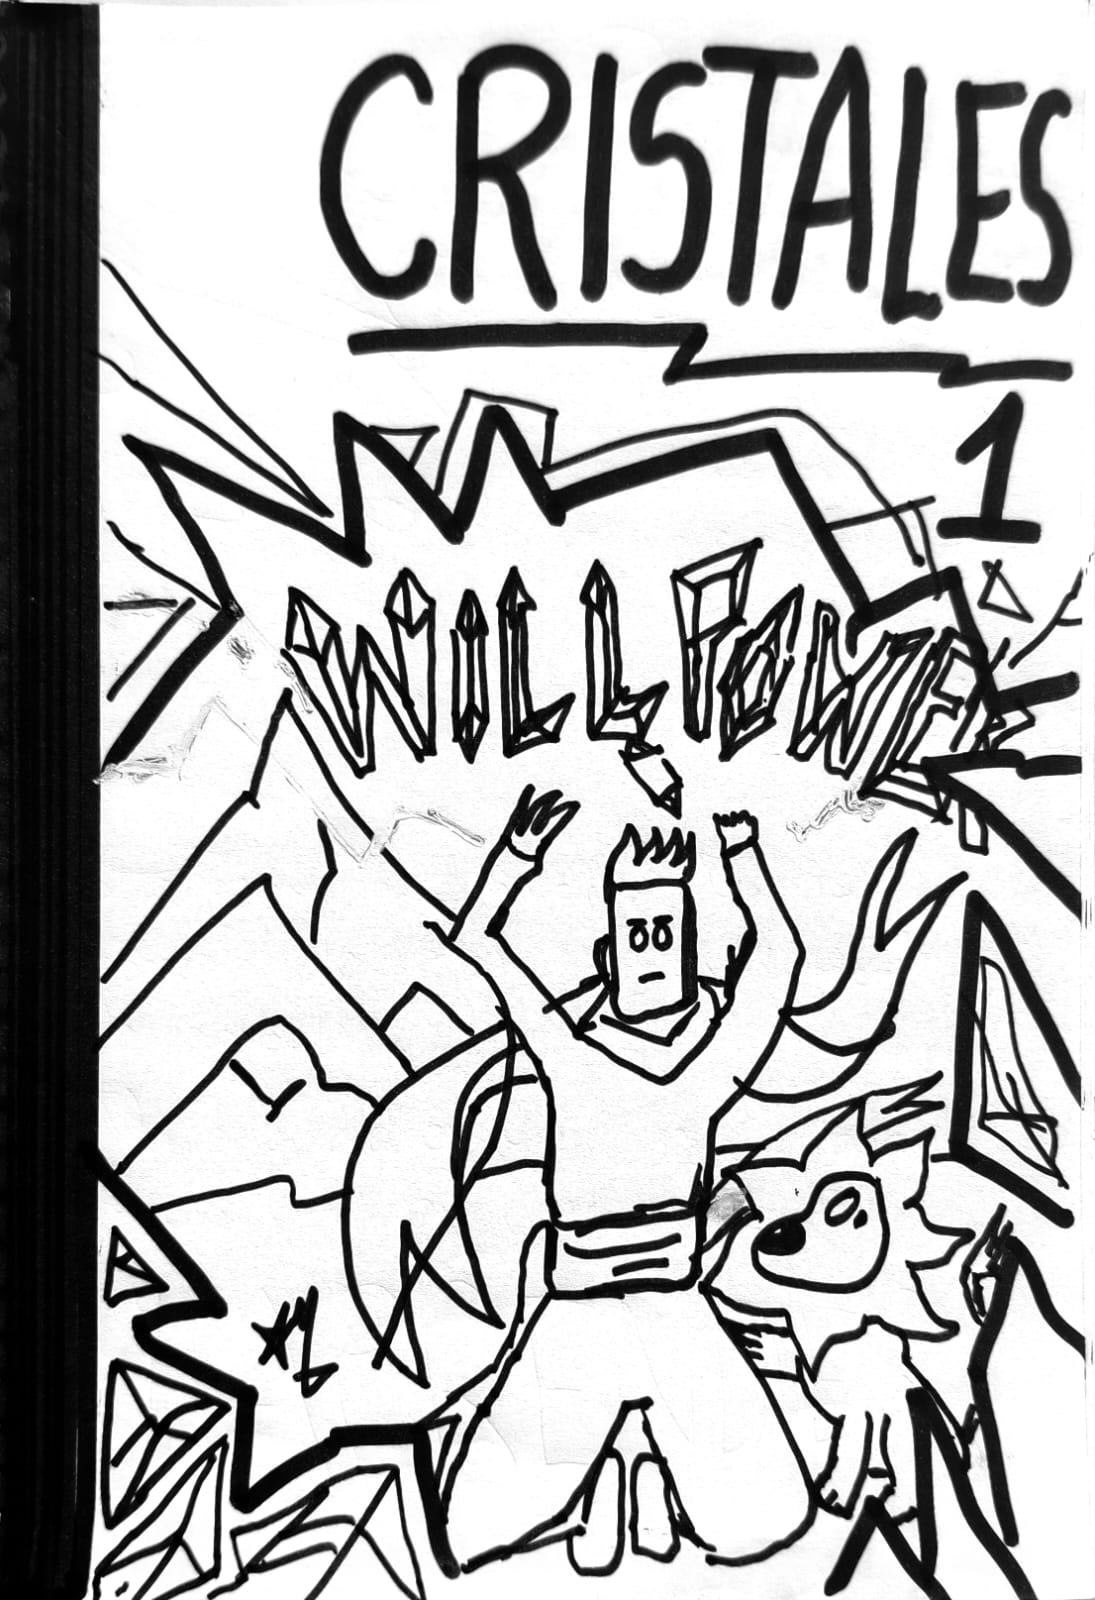
\includegraphics[width=\paperwidth,height=\paperheight]{images/portada1.jpeg}}%
}
\thispagestyle{empty}
\null
\clearpage

% --- Advertencia ---
\thispagestyle{empty}
\vspace*{\fill}
\begin{center}
\hazardstripe

\vspace{7mm}
{\fontsize{55}{55}\selectfont\faExclamationTriangle}

\vspace{5mm}
{\sffamily\bfseries\fontsize{34}{38}\selectfont ADVERTENCIA}

\vspace{9mm}
\begin{minipage}{0.85\linewidth}
\centering\sffamily\bfseries\large
DECLARO QUE ESTE LIBRO ES PARA MAYORES DE 18 AÑOS Y TODO AQUEL MENOR DE EDAD QUE ESTÉ DISPUESTO A CUESTIONAR SU IDENTIDAD.
\end{minipage}

\vspace{9mm}
\hazardstripe
\end{center}
\vspace*{\fill}
\clearpage

\tableofcontents

\mainmatter

\renewcommand{\chaptertitlename}{Chapter}
\chapter{Star: The End of the Beginning}
\renewcommand{\chaptertitlename}{Capítulo}

\nowplaying{1303 Passacaglia}{SynthWulf}

\lettrine{R}{ápido}, sigue corriendo, esquiva, salta, agáchate, corre, pero no pares, descubre, alerta, cuidado, sigue avanzando. Duda, acepta, cuidado pero sigue corriendo ``Cuántas formas de comenzar una historia y decidí hacerlo de esta forma, eso es GENIAL'', porque yo lo elegí, yo la creé, y eso la volverá única en el mundo.

Alerta, ¡estamos bajo ataque!, sigue corriendo, sé consciente, decide tu moral, ¡crea tu realidad!, confía, ama, ve a los bosques y descubre si realmente has llegado a conocer aquello llamado vida.

Todo será increíble, pero tendré que pagar el riesgo, tendré que pagar el esfuerzo.

Corre, no pares de avanzar, tropiezo, pero no me detengo, sigue avanzando, baila, ríe, llora, confía, desconfía, sé lógico, sé amado, ama, descubre tu identidad, constrúyela.

Todos son invitados a participar, todos son invitados a ganar, pero asuma las consecuencias de sus actos. Si no le gustan cómo están las cosas, USTED es quien debe cambiarlas, y si no está dispuesto a hacer el esfuerzo necesario para cambiarlas, entonces, ¡NO SE QUEJE!

¿En dónde estoy? ¿Quién soy? Si puedo pensar, ¿soy un ser consciente, verdad? Espera, claro, si puedo transformar mi pensar en palabras, debo ser un ser pensante.

¡Alerta!, aquí hay seres también, aquí hay seres como yo, ¿qué es lo que cae?, rápido, debo ser yo mismo.

Correr me hace sentir vivo, correr me hace sentir feliz.

Correr me hace sentir feliz.
Correr me hace sentirme yo mismo.

Correr dibuja una sonrisa en mi rostro.

¿Qué sucede, qué es todo aquello que cae, qué es eso que destruye mi felicidad, qué es\ldots?

Todo está siendo destrozado. Si no cuido de mí, nadie lo hará por mí, esquivo, salto, danzo, la forma en cómo interprete esta situación definirá el rumbo de mi destino, definirá mi proceder. No soy el único que está aterrado. Cada ser corre de su interpretación.

Corre, no mires atrás, pude haber intentado salvarlos, pero ¿quién me salvará a mí?, cuidado.

¿Por qué no hice nada? ¿Por qué no salvé su situación?
¿Fue por miedo?

¿El miedo es una excusa lo suficientemente fuerte para impedirme actuar?
Tantas cosas que pudo ser y no hice más que observar, si solo pudiera retroceder el tiempo, cuántas cosas pasan por mi mente de todo lo que pudo ser, ¡es fácil crear el mejor escenario!, es fácil crear todo lo que pudo haber sido.

Hay un ser ahí, que se inmuta ante el caos, tengo la oportunidad de salvarlo, puedo influir en su vida.

¡Pude actuar, esta vez! ¡Pude actuar! No me quedé parado, ni fui un simple espectador, PUDE ACTUAR, fue gracias a las veces que no actué que pude actuar en esta ocasión. ¿Qué más podré hacer? No es momento de pensar, no es momento de lamentar. Mi prioridad es vivir, mi prioridad es descubrir, mi prioridad es APRENDER.

\renewcommand{\chaptertitlename}{Chapter}
\chapter{Star: Are you okey?}
\renewcommand{\chaptertitlename}{Capítulo}

\nowplaying{KILLSWITCH (Levia Remix)}{mekaloton \& Levia}

\lettrine{B}{usco} tu mirada entre el polvo y el ruido. —¿Estás bien? Hey, ¿qué tal, mi pequeño felino? ¿Te encuentras bien?

El cielo se parte en pedazos de fuego: meteoritos con forma de estrella caen hacia nosotros a una velocidad que no debería existir. El rostro de León cambia, y por primera vez desde que lo conozco, veo miedo dibujado en él.

\illustration{images/Chapter-1/leon-asustado.png}{León, aterrado, ve caer los meteoritos por primera vez.}

—¿Qué sucede? ¿Por qué tu rostro cambió así? ¿Por qué tienes miedo?

No hay tiempo para respuesta. Uno de los meteoritos cae directo hacia mí y León me empuja con todo su peso, apartándome del impacto.

\illustration{images/Chapter-1/leon-super-asustado.png}{El instante justo después de empujar a Jhonny fuera de peligro.}

—¡Auch! ¿Por qué hiciste eso? —Ya entiendo. Esto no va a parar. Siguen cayendo, una tras otra. Rápido, corre conmigo.

Tal vez, para ayudar a otros, deba ayudarme primero a mí mismo.

A lo lejos, entre gritos, alguien menciona un «amuleto encantado». Esquivamos como podemos, con una coreografía improvisada de saltos y giros que se siente casi elegante, casi \emph{cool}, aunque yo todavía no tengo ningún poder. Solo sé esquivar.

Wow. Así que esta es mi condición física real. ¿Por qué no me ejercité cuando pude? ¿Por qué no cuidé mi cuerpo cuando era el momento? ¿Qué edad tengo? ¿En dónde estoy?

Alguien pasa corriendo a una velocidad imposible y me grita sin detenerse: \emph{``You're too slow.''}

Una chica corre a mi lado, hablando más para sí misma que para mí: —Esto no hubiera pasado si hubiera continuado mis estudios en la San Marino.

Tropiezo. León me carga sobre su espalda sin detener el paso. Algo me lanza una telaraña directo a la boca; la escupo, desorientado. ¿Dónde estoy?

Corremos en dirección contraria a los meteoritos, hacia un muro enorme que divide lo que aún se puede cruzar de lo que ya no.

A mi izquierda, un niño le grita a su robot que busque en su bolsillo algo que los pueda sacar con vida de ahí. El robot obedece: de un bolsillo diminuto empiezan a salir objetos que no deberían caber, uno tras otro, imposibles.

A mi derecha, un ser dibuja círculos en el suelo junto a una armadura metálica que convierte el piso mismo en un vehículo.

Todo el mundo está improvisando su propia forma de sobrevivir. Yo solo sé correr. Y esquivar. Y preguntarme, mientras el cielo sigue cayendo, cuánto tiempo más podré seguir haciendo solamente eso.


\backmatter

% --- Créditos musicales ---
\chapter*{Créditos musicales}
\addcontentsline{toc}{chapter}{Créditos musicales}

\emph{Las canciones mencionadas a lo largo de este libro son sugerencias de acompañamiento para la lectura. Todos los derechos de autor pertenecen a sus respectivos artistas, compositores y sellos discográficos. Este libro no reclama ninguna propiedad sobre dichas obras; se mencionan únicamente con fines de recomendación.}

\bigskip

% Agregar una entrada por cada capítulo que use \nowplaying
\noindent\textbf{Chapter 1 --- Star: El final del inicio}\\
1303 Passacaglia --- SynthWulf

\bigskip

\noindent\textbf{Chapter 2 --- Star: Are you okey?}\\
KILLSWITCH (Levia Remix) --- mekaloton \& Levia

\end{document}